\iffalse

\chapter{Fundamentarea teoretică și documentarea bibliografică}
\label{cap:cap1}

(10–15 pagini)\footnote{Template-ul a fost construit similar celui dezvoltat de George VIERIU, disponibil la \url{https://ac.tuiasi.ro/studenti/didactic/finalizare-studii/finalizare-studii-calculatoare/finalizare-studii-calculatoare-ghidul-studentului/}}

\begin{itemize}
    \item Domeniul și contextul abordării temei;
    \item Tema propusă (formularea exactă a temei, obiective, justificarea abordării);
    \item Prezentare succintă și comparativă privind realizările actuale pe aceeași temă;
    \item Analiza tipurilor de produse/aplicații existente din respectiva categorie a temei,
tehnologii folosite pentru implementare;
    \item Elaborarea specificațiilor privind caracteristicile așteptate de la aplicație. 
\end{itemize}

Lucrările utilizate în dezvoltarea proiectului de diplomă și în redactarea tezei vor fi citate corespunzător în cadrul prezentului document. Această citare trebuie să fie o interpretare sau o descriere proprie autorului prezentei teze asupra ideii/soluției/conceptului prezentat în lucrarea sursă și \textbf{\textit{nu}} o preluare mot-a-mot sau o traducere directă. O posibilă excepție de la această regulă se poate face în cazul rezultatelor teoretice importante, cum ar fi, de exemplu, definițiile, teoremele sau algoritmii suport. În textul asociat citării este recomandat să includeți, de asemenea, și o frază prin care să realizați legătura cu lucrarea proprie. Teza capătă în acest fel consistență și evitați ideea de citare bulk, „doar ca să fie". În continuare vă prezentăm un scurt exemplu.

\todo[inline]{TO DO: Aici ar trebui să introduc o referință bibliografică deoarece ceea ce am scris nu este ideea mea}

Mironeanu et. al. propun o nouă abordare pentru monitorizarea și prevenția atacurilor cibernetice \cite{art:mironeanu:ECAD:2021}. Soluția utilizează tehnici de tip AI/ML și pe un sistem de votare ponderat cu scopul de determina dacă un acces în rețea este un acces normal sau un eventual atac. Pornind de la noțiunile descrise în \cite{art:mironeanu:ECAD:2021}, lucrarea de față își propune îmbunătățirea detecției atacurilor de tip \textit{flood}.

Pornind de la modelul REST propus de Fielding în \cite{thesis:fielding:2000} și considerând specificațiile protocolului HTTP \cite{misc:web:rfc7231}, Archip et. al. demonstrează în \cite{inproc:archip:restful:2018} faptul că o utilizare greșită a modelului amintit poate conduce la o slăbire a securității unui server. Un alt aspect important care trebuie considerat cu privire la securitatea sistemelor informatice este legat de utilizatori. Acest subiect este tratat pe larg în \cite{incollection:ARASEC2020}.

Un exemplu de intrare bibliografică pentru un \textit{tech report} este în \cite[p.~13]{IEEEexample:techreptypeii} (numărul paginii este trecut explicit în sursă). Bineînțeles, nu putem discuta despre configurările și instalările unor sisteme Cloud Computing \cite[p.~113]{book:marinescu:2018}, dacă nu considerăm și sistemele de operare suport sau gazdă \cite{book:operating_systems:2014}. În cazul în care dorim să referim o pagină web care nu se încadrează în categoriile carte, articol, raport tehnic, putem să utilizăm o intrare de tip \verb|misc| în bibliografie. Recomandarea este să utilizăm documente Web publicate de companii importante (precum IBM, RedHat, Apple, etc.) sau personalități recunoscute, precum Bruce Schneier \cite{misc:web:schneier2021}.

\textcolor{gray}{\lipsum}(Figura \ref{fig:puterea_furnizata_pe_cm_cub})

\begin{figure}[H]
    \centering
    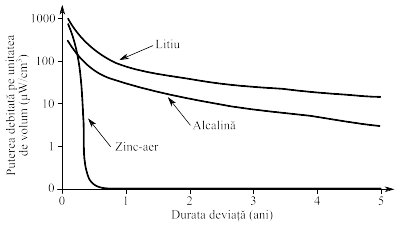
\includegraphics[width=0.6\textwidth]{continut/capitol1/figuri/puterea_furnizata_pe_cm_cub.png}
    \caption{Puterea furnizată pe cm\textsuperscript{3} relativă la durata de viață pentru trei tipuri de baterii.}
    \label{fig:puterea_furnizata_pe_cm_cub}
\end{figure}

\textcolor{gray}{\lipsum}

\section{Exemplu de subcapitol nivel 1}
\label{cap:cap1:ex-subcapitol}

\textcolor{gray}{\lipsum} (Figura \ref{fig:r2_d2})

\begin{figure}[t]
    \centering
    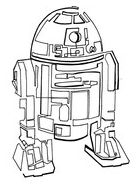
\includegraphics[width=0.25\textwidth]{continut/capitol1/figuri/r2_d2.png}
    \caption{R2-D2\protect\footnotemark}
    \label{fig:r2_d2}
\end{figure}
\footnotetext{imagine preluată de pe un site web care nu „merită” trecut la bibliografie \url{https://www.shutterstock.com/}}

\textcolor{gray}{\lipsum} 

\subsection{Exemplu de subcapitol nivel 2}
\label{cap:cap1:ex-supcapitol:nivel2}

\textcolor{gray}{\lipsum} (Figura \ref{fig:yoda})

\begin{figure}[H]
    \centering
    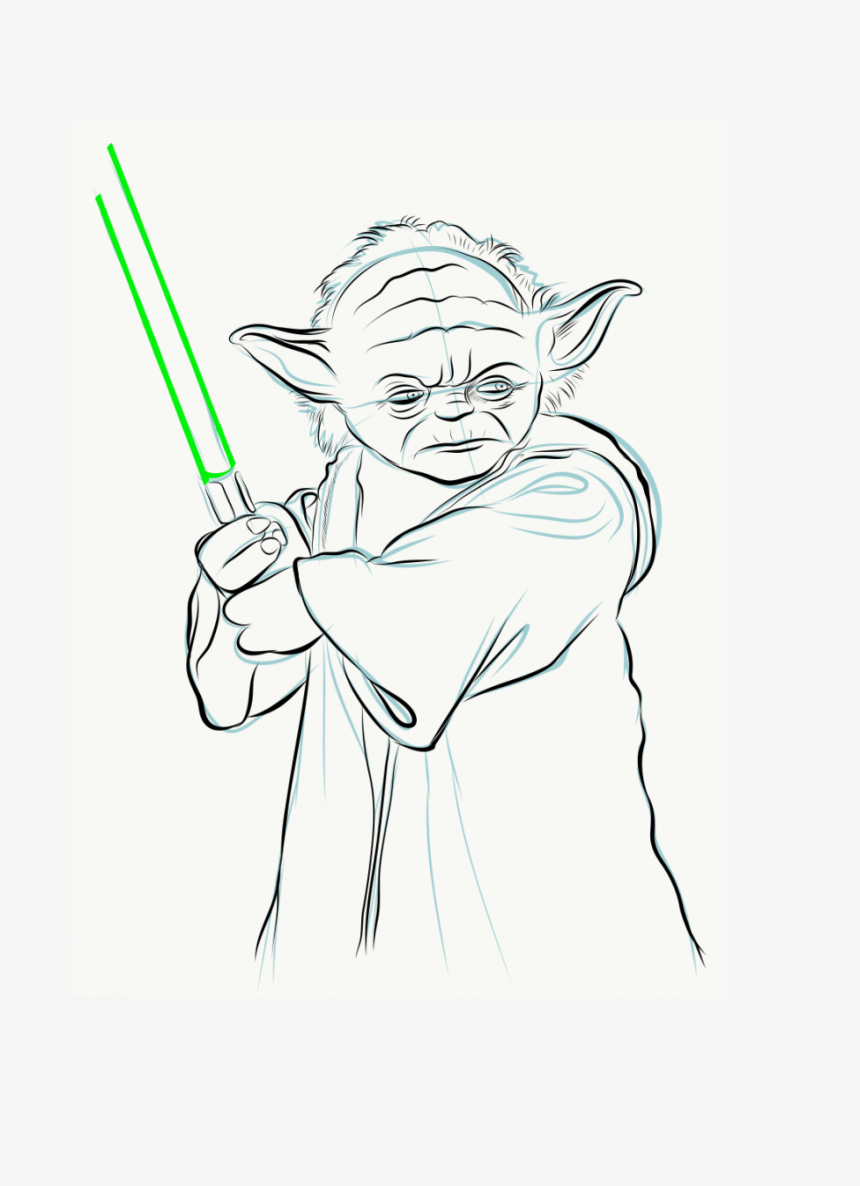
\includegraphics[width=0.3\textwidth]{continut/capitol1/figuri/yoda.png}
    \caption{Yoda\protect\footnotemark}
    \label{fig:yoda}
\end{figure}
\footnotetext{imagine preluată de pe un site web care nu „merită” trecut la bibliografie \url{https://www.pngitem.com/}}

\textcolor{gray}{\lipsum}

\subsubsection{Exemplu de subcapitol nivel 3}
\label{cap:cap1:ex-subcapitol:nivel2:nivel3}

\textcolor{gray}{\lipsum}

Următoarele e fără label FTW, decât să demonstrez gen!\footnote{Dacă vă prindem cu astfel de exprimări, vă scădem 2 puncte!!!}

\section{Nivel 1}
\label{cap:cap1:nivel1}

\subsection{Nivel 2}
\label{cap:cap1:nivel1:nivel2}

Ghilimelele se pun înainte și după reproducerea unui text. Se pun între semnele citării cuvintele sau grupurile de cuvinte citate ironic sau care redau atitudinea rezervată ori dezaprobatoare a autorului față de realitățile pe care le desemnează respectivele cuvinte. Se obișnuiește să se pună între ghilimele titlurile operelor literare de artă sau științifice, ale publicațiilor, numele instituțiilor, firmelor etc. atunci când aceste titluri sunt reproduse într-o frază. 
Atenție: Ghilimelele limbii engleze (“ ”) sunt diferite de ghilimelele limbii române („ ”)!
Observație: Documentele tehnice au adoptat din sintaxa limbajelor de programare ghilimelele duble (") pentru a evidenția șirurile de caractere în text și ghilimelele simple (') pentru evidențierea caracterelor. De exemplu: "acesta este un șir de caractere", acesta este caracterul 'x'.

\subsubsection{Nivel 3}
\label{cap:cap1:nivel1:nivel2:nivel3}

Oricum, mai departe de \verb|#.#.#.#| \textbf{\textit{NU}} trebuie să se ajungă :P.

\fi


\chapter{Fundamentarea teoretică și documentarea bibliografică}
\label{cap:cap1}

Structura următoarelor câteva subcapitole este puternic influențată de structura cursului de Calcul Cuantic din cadrul Facultății de Informatică de la Universitatea "Alexandru Ioan Cuza", predat de doamna Conf. Arusoaie Andreea, fără de care această lucrare probabil că nu ar fi fost posibilă. Voi încerca a prezenta doar elementele relevante, pe scurt, pentru această lucrare, rezumând / scurtând / eliminând acele elemente care nu vor avea nici o legătură cu lucrarea.

\section{Elemente de algebră liniară}

\subsection{Mulțimea numerelor complexe}

Mulțimea numerelor complexe este un sistem de numărare care conține numerele reale și o unitate imaginară $i$ care îndeplinește proprietatea:
\[i^2 = -1\]
Uneori, definiția unității imaginare este dată in literatura de specialitate ca fiind: \[i = \sqrt{-1}\]
Se numește număr complex orice număr de forma \[z = a + ib,\] unde $a$ și $b$ sunt numere reale. Mulțimea numerelor complexe $\mathbb{C}$ este așadar definită în felul următor: 
\[ \mathbb{C} = \{z \enspace|\; z = a + ib,\enspace a,\enspace b \enspace\in\enspace \mathbb{R},\enspace i^2 = -1\} \]

Conjugatul unui număr complex $z$ este definit ca:
\[\bar{z} \overset{not.}{=} z\text{*} = a - ib\]
Notația cu bară deasupra pentru $z$ este deseori utilizată în matematică, iar notația cu asterisc este utilizată mai des în fizică. Pe parcursul acestei lucrări se vor folosi oarecum interschimbabil cele două notații datorită gamei largi de surse de studiu (cărți, cursuri din diferite spații culturale / academice ș.a.m.d.)

Modulul sau amplitudinea unui număr complex:
\[z = \sqrt{a^2 + b^2}\]

\textbf{Proprietăți ale numerelor complexe}:

Fie $z, w \in \mathbb{C}$. Atunci au loc:
\begin{itemize}
    \item $\overline{z + w} = \bar{z} + \bar{w}$ 
    \item $z \cdot \bar{z} = \bar{z} \cdot z = |z|^2$
    \item $\bar{\bar{z}} = z$
    \item $|z| = |\bar{z}|$
\end{itemize}
\newpage

Forma trigonometrică a numerelor complexe este dată de formula:
\[z = A(\cos \theta + i \sin \theta) = Ae^{i\theta}\] 

Unde $A = \sqrt{a^2 + b^2}$,  $\theta = \arctan\left(\dfrac{b}{a}\right)$

\subsection{Spații vectoriale}
Fie $V \neq \phi$ și $K$ un corp comutativ peste $\mathbb{R}$ sau $\mathbb{C}$. Un corp este un triplet $(K, +, *)$ în care $K$ este o mulțime cu cel puțin două elemente, iar $+$ și $*$ doi operatori satisfăcând următoarele axiome:
\begin{itemize}
    \item $(K,+)$ este un grup abelian cu un element neutru $0$.
    \item $(K \setminus \{0\}, *)$ este grup cu un element neutru $1$.
    \item Operatorul $*$ este distributiv față de operatorul $+$.
\end{itemize}

Dacă în plus operatorul $*$ este comutativ (adică axioma doi implică conceptul de \textit{grup abelian}), atunci spunem că tripletul $(K, +, *)$ este \textit{corp comutativ}.

Un grup este o mulțime prevăzută cu un operator care combină orice două elemente ale ei pentru a forma un al treilea element în așa fel încât sunt satisfăcute patru condiții, denumite axiomele grupurilor.

Se numește spațiu liniar (sau vectorial) peste K, o mulțime V, inzestrată cu:
\begin{itemize}
    \item \textit{o lege internă} $\enspace+$: \enspace$V \times V \rightarrow V,\enspace (x, y) \rightarrow x + y,\enspace \forall x,y \in V$,
    \item \textit{o lege externă} $\enspace\cdot$: $K \times V \rightarrow V, \enspace (\alpha, x) \rightarrow \alpha \cdot x, \enspace \forall \alpha \in K, x \in V$, 
\end{itemize}

Astfel încât sunt îndeplinite următoarele axiome:

\begin{itemize}
    \item $x + (y + z) = (x + y) + z,  \enspace \forall x,y,z \in V$,
    \item $x + y = y + x, \enspace \forall x, y \in V$,
    \item $\exists0 \in V, \forall x \in V: x + 0 = 0 + x = x$,
    \item $\forall x \in V, \exists (-x) \in V: x + (-x) = (-x) + x = 0$,
    \item $\alpha \cdot (x+y) = \alpha \cdot x + \alpha \cdot y, \forall \alpha \in K, x,y \in V$,
    \item $(\alpha + \beta)\cot x = \alpha \cdot x + \beta \cdot y\ forall \alpha, \beta \in K, x \in V$,
    \item $\alpha \cdot (\beta \cdot x) = (\alpha \beta ) \cdot x, \forall \alpha, \beta \in K, x \in V$,
    \item $1 \cdot x = x, \forall x \in $, unde 1 este elementul unitate din K.
\end{itemize}

Elementele aparținând spațiului liniar $V$ sunt numite vectori, iar elementele aparținând lui $K$ se numesc scalari. Deseori, pentru "legile" interne / externe definite mai sus se folosesc denumirile de "adunarea vectorilor" pentru "+", respectiv "multiplicarea vectorului cu scalar" pentru "$\cdot$". Un element 0 $\in V$ se numește vector nul. În cazul în care $K = \mathbb{R}$, atunci V se numește spațiu liniar real, iar în cazul în care $K = \mathbb{C}$, atunci V se numește spațiu liniar complex. 
Întotdeauna, spațiul stărilor unui sistem cuantic este descris în termenii unui spațiu liniar complex.

În cadrul acestei lucrări, vectorii vor fi considerați a fi în formă \textit{coloană}, adică vor fi scriși în felul următor:
\[
\begin{bmatrix}
1 \\ 2
\end{bmatrix}
\]
dar, de dragul lizibilității vor fi scriși în rând cu textul sub forma (1, 2). În acest caz, se consideră a fi în continuare sub formă coloană.

Fie $\forall n \in \mathbb{N}\text{*}$.

Atunci $\mathbb{C}^n = \mathbb{C} \times \mathbb{C} \times ... \times \mathbb{C}$. Dacă $u \in \mathbb{C}^n, u=(u1, u2, ..., un) \overset{not.}{=} \begin{bmatrix}
u1 \\ u2 \\ ... \\ un
\end{bmatrix}, ui \in \mathbb{C}$.

Atunci, în concluzie, $(\mathbb{C}^n, +, \cdot, \mathbb{C})$ este spațiul vectorial complex adus în discuție anterior, util pentru descrierea spațiului stărilor unui sistem cuantic.

\subsection{Spațiu euclidian complex}

Fie $V$ un spațiu liniar peste $\mathbb{C}$. Se numește produs scalar complex funcția $\braket{\cdot, \cdot}: V \times V \rightarrow \mathbb{C}$ cu proprietățile:
\begin{itemize}
    \item $\braket{u,u} \geq 0, \forall u \in V$,
    \item $\braket{u,u} = 0, \iff u = 0$,
    \item $\braket{u,v} = \overline{\braket{v, u}}, \forall u, v \in V$,
    \item $\braket{u, \alpha v + \alpha ' v '} = \alpha \braket{u, v} + \alpha ' \braket{u ', v}, \forall \alpha, \alpha ' \in \mathbb{C}, u, u ' , v \in V$,
    \item $\braket{\alpha u, v} = \bar{\alpha} \braket{u, v}, \alpha \in \mathbb{C}$.
\end{itemize}

Un spațiu liniar peste $\mathbb{C}$ înzestrat cu produs scalar se numește spațiu euclidian complex sau spațiu prehilbertian.

Produsul scalar a vectorilor $u, v \in \mathbb{C}^n$ este definit prin:
\[
    \braket{u,v} = \sum_{i=0}^{n} \bar{u_i v_i}, \enspace u_i, v_i \in \mathbb{C}
\]
În fizica cuantică, o stare a unui sistem este reprezentată de un vector dintr-un spațiu Hilbert, adică un spațiu vectorial complex dotat cu un produs scalar.

Norma euclidiană a vectorului $u \in \mathbb{C}^n$ este definită prin:
\[
||u|| = \sqrt{\braket{u,u}} = \sqrt{\sum_{i=1}^{n} |u_i|^2}.
\]

\subsection{Baze ortonormale}

Fie $V$ un spațiu euclidian de dimensiune $n$ și fie $B = \{b_1, b_2, ... , b_n\}$ o bază.

$B \subset V$ se numește \textit{bază} a spațiului $V$ dacă $B$ este liniar independentă și Span(B) = V, unde mulțimea Span(U) a unui spațiu euclidian U este definită prin  \[Span(U) =\sum_{i=1}^{n} \alpha_i u_i, \enspace n \in \mathbb{N}\text{*}, u_1, ... u_n \in U\] iar iar elementele $u_1, ..., u_n$ se numesc liniar independente dacă ecuația \[\beta_1 u_1 + ... + \beta_n u_n =0\], are soluție unică$\beta_1 = ... = \beta_n = 0$.


Pentru $\forall u, v \in V$, are loc 
\[
u = \sum_{i=1}^{n} u_i b_i, \enspace v = \sum_{i=1}^n v_i b_i,
\]
iar expresia produsului scalar este 
\[
\braket{u, v} = \sum_{i=1}^{n} \sum_{j=1}^{n} u_i v_j \braket{b_i, b_j}.
\]
Spunem că baza B este \textit{bază ortonormală} dacă
\[
\braket{b_i, b_j} =
\begin{cases}
0, \enspace i \neq j, \\
1, \enspace i = j.
\end{cases}
\]

\subsection{Operatori liniari. Conjugata. Transpusa.}

Fie $\mathcal{L}(X, Y)$ mulțimea operatorilor liniari X cu valori în Y, unde noțiunea de \textit{operator liniar} înseamnă orice aplicație $A: X \rightarrow Y$ unde 
\[
A (\alpha x + \beta y) = \alpha A(x) + \beta A(y), \enspace \forall \alpha, \beta \in \mathbb{C}, \enspace x, y \in X.
\]

Fie $X = \mathbb{C}^m$ și $Y = \mathbb{C}^n$ și fie $A \in \mathcal{L}(X,Y)$.
Operatorul \textit{conjugat} $\bar{A} \in \mathcal{L}(X, Y)$ are matricea asociată definită prin
\[
\bar{A}(i,j) = \overline{A(i,j)}, i \in \{1, ..., m\}, j \in \{1, ..., n\}
\]
Operatorul \textit{transpus} $A^T \in \mathcal{L}(X, Y)$ este operatorul ce are matricea asociată
\[
A^T(i,j) = A(j,i).
\]


\section{Tranziția către calcul cuantic}
\subsection{Notația bra ket (Dirac)}

Voi prezenta puțin mai târziu postulatele mecanicii cuantice, printre care se numără și definiția unui \textit{bit cuantic}, sau \textit{qubit}, dar deocamdată aș dori să prezint notația bra-ket pentru vectori de stare, utilizați intens în următoarele secțiuni. 

Deseori, starea unui qubit este reprezentat de un versor din spațiul de două elemente complexe:
\[
\ket{\psi} = \begin{bmatrix} \alpha \\ \beta \end{bmatrix} \in \mathbb{C}^2,
\]
unde $\alpha, \beta \in \mathbb{C}$. Așadar, $\ket{\cdot}$ - notația \textit{ket} a vectorilor de stare.

Pentru același $\psi$ definit mai sus, definim 
\[
\bra{\psi} = \overline{(\ket{\psi})^T} = \begin{bmatrix}
\bar{\alpha} \bar{\beta}
\end{bmatrix}
\]
Deci, $\bra{\cdot}$ - notația \textit{bra} a vectorilor de stare, care e pur și simplu conjugata transpusă a vectorului de stare scris în notația ket.

\subsection{Produsul scalar pentru spațiul vectorial complex}
Un produs scalar pe un spațiu vectorial complex $V$ este o operație ce asociează fiecărei perechi de vectori $\bra{u}$, $\bra{v}$ un număr complex
\[
\braket{u|v} = \braket{\ket{u}, \ket{v}} = \sum_{i=1}^{n} \bar{u_i}v_i
\]

\subsection{Operatorul adjunct}
Fie $A$ un operator liniar pe un spațiu vectorial $V$. Atunci, există un unic operator $A^\dagger$ pe V astfel încât $\forall \ket{v}, \ket{w} \in V$ să avem
\[
    \braket{v|Aw} = \braket{A^\dagger v | w}.
\]
Operatorul liniar $A^\dagger$ se numește operatorul adjunct al lui A (citit deseori și ca "dagger").
În termeni matriceali, $A^\dagger = \overline{A^T}$, unde $\overline{A^T}$ reprezintă conjugata matricei A, transpuse.
Pentru același $\ket{\psi}$ definit în prima subsecție a acestei secții, $\ket{\psi}^\dagger = \bra{\psi} = \overline{\ket{\psi}^T}$.

\subsubsection{Proprietăți ale operatorului adjunct}

Fie $V$ un spațiu Hilbert de dimensiune $n$.
Spunem că operatorul (matricea) A este normal dacă
\[
AA^\dagger = A^\dagger A;
\]
Spunem că operatorul A este hermitian sau autoadjunct dacă 
\[
A = A^\dagger
\]
Spunem că un operator A este \textit{unitar} dacă
\[
A A^\dagger = A^\dagger A = I_n
\]
Operatorii unitari satisfac:
\[
\braket{Au|Av} = \braket{u|v}.
\]

Aceste lucruri vor fi foarte importante când voi prezenta conceptul de \textit{poartă logică cuantică} în următoarele secțiuni.

\subsection{Produsul tensorial}

Fie $U, V$ două spații Hilbert de dimensiune $m$, respectiv $n$. Atunci, produsul tensorial $U \otimes V$ este un spațiu Hilbert, de dimensiune $m \cdot n$.

Pentru doi vectori de stare $\ket{\psi_1} \in U$ și $\ket{\psi_2} \in V$, produsul tensorial este un vector $\ket{\psi_1} \otimes \ket{psi_2}$ din $U \otimes V$.

Dacă A și B sunt doi operatori (matrice) liniari pe $U$, respectiv $V$, atunci $A \otimes B$ este un operator liniar peste $U \otimes V$ definit prin
\[
(A \otimes B) (\ket{\psi_1} \otimes \ket{\psi_2}) \equiv A \ket{\psi_1} \otimes B \ket{\psi_2}
\]

\subsubsection{Reprezentarea matriceală}

Pentru două matrice 
\[
A = \begin{bmatrix}
a_{11} & a_{12} \\
a_{21} & a_{22}
\end{bmatrix}
\]
\[
B = \begin{bmatrix}
b_{11} & b_{12} \\
b_{21} & b_{21}
\end{bmatrix}
\]

Produsul tensorial $A \otimes B$ este definit prin:
\[
A \otimes B = \begin{bmatrix}
a_{11}B & a_{12}B \\
a_{21}B & a_{22}B
\end{bmatrix},
\]
unde $a_{ij}B$ reprezintă înmulțirea matricei B cu un scalar $\implies$ matricea rezultată produsului scalar va fi de dimensiune $4 \times 4$.


\section{Calcul cuantic}

\subsection{Postulatele mecanicii cuantice, din perspectiva calculului cuantic}

În următoarele câteva subsecțiuni voi oferi o perspectivă de ansamblu asupra celor patru postulate ale mecanicii cuantice prezentate de Nielsen și Chuang in \cite{book:QCQI10E:2011}. Voi încerca să combin explicațiile din capitolul 2 a primei părți a cărții cu cele din primul capitol, cu excepția celor despre porți logice cuantice și circuite cuantice, pe care le voi explica după ce termin perspectiva asupra postulatelor mecanicii cuantice, în același fel în care a organizat și doamna Conf. Arusoaie cursul de Quantum Computing menționat anterior.

\subsubsection{\textbf{Postulatul I} - Definiția unui qubit}

Enunțul postulatului este următorul: "Există un spațiu vectorial complex dotat cu produs tensorial (adică, un spațiu Hilbert) asociat oricărui sistem fizic cuantic izolat, cunoscut drept spațiul stărilor a sistemului. Sistemul este descris în totalitate de către vectorul stărilor sale, care este un vector unitar în spațiul stărilor sistemului".

Într-o altă formă, am regăsit enunțul acestui postulat și sub forma următoare: "Oricărei stări fizice posibile a unui sistem cuantic îi corespunde un versor (vector de mărime 1) dintr-un spațiu vectorial complex, dotat cu un produs scalar (spațiu Hilbert)".

Cel mai important lucru este faptul că starea unui sistem fizic cuantic (în cazul ) este descrisă de un versor, numit \textit{vector de stare}. 

Fie $\ket{0}, \ket{1} \in \mathbb{C}$. Atunci definim:

\[
\ket{0} = \begin{bmatrix}
1 \\ 0
\end{bmatrix}
\enspace
\ket{1} = \begin{bmatrix}
0 \\ 1
\end{bmatrix}
\]

Atunci, mulțimea {$\ket{1}, \ket{0}$} este o bază ortonormală a lui $\mathbb{C}^2$. Așadar, orice vector de stare din spațiul stărilor poate fi scris ca o combinație liniară de stări $\ket{0}$ și $\ket{1}$, notat
\[
\ket{\psi} = \alpha\ket{0} + \beta\ket{1},
\]
unde $\alpha$ și $\beta$ sunt numere complexe, uneori numite și "amplitudini cuantice".

În plus, cum starea $\ket{\psi}$ este un versor, satisface proprietatea $||\ket{\psi}|| = 1$, adică
\[
\sqrt{\braket{\psi|\psi}} = 1 \implies |\alpha|^2 + |\beta|^2 = 1.
\]

Așadar, vom numi starea $\ket{\psi}$ drept \textit{bit cuantic}, sau \textit{qubit}.

\subsubsection{Reprezentarea geometrică a qubitului}

Din proprietatea $|\alpha|^2 + |\beta|^2 = 1$ menționată anterior, putem rescrie ecuația sub forma 
\[
\ket{\psi} = e^{i\gamma}(\cos \frac{\theta}{2}\ket{0} + e^{i\varphi}\sin\frac{\theta}{2}\ket{1}),
\]

unde $\theta, \varphi, \gamma$ sunt numere reale. Din cauza unor motive pe care nu le voi detalia aici, factorul $e^{i\gamma}$ din față poate fi eliminat, deoarece nu are nici un efect observabil. Din acest motiv, putem scrie:
\[
\ket{\psi} = \cos \frac{\theta}{2} + e^{i\varphi}\sin \frac{\theta}{2}\ket{1}.
\]

Cum numerele reale $\theta$ și $\varphi$ definesc un punct pe sfera unitate tridimensională, putem folosi o reprezentare numită "sfera Bloch" pentru starea unui bit cuantic. Aceasta este o metodă foarte utilă pentru vizualizarea unui singur bit cuantic, dar din păcate nu există o generalizare trivială a sferei Bloch pentru qubiți multipli. 

\begin{figure}[H]
\centering
    \caption{O sferă Bloch cu un vector $\ket{\psi}$ oarecare și unghiurile $\theta$ și $\varphi$}
    \label{fig:BlochOarecare}
\begin{tikzpicture}


    % Define radius
    \def\r{4}

    % Bloch vector
    \draw (0,0) node[circle,fill,inner sep=1] (orig) {} -- (\r/3,\r/2) node[circle,fill,inner sep=0.7,label=above:$\ket{\psi}$] (a) {};
    \draw[dashed] (orig) -- (\r/3,-\r/5) node (phi) {} -- (a);

    % Sphere
    \draw (orig) circle (\r);
    \draw[dashed] (orig) ellipse (\r{} and \r/3);

    % Axes
    \draw[->] (orig) -- ++(-\r/5,-\r/3) node[below] (x) {$x$};
    \draw[->] (orig) -- ++(\r+0.5,0) node[right] (y) {$y$};
    \draw[->] (orig) -- ++(0,\r+0.5) node[above] (z) {$z$};

    %Angles
    \pic [draw=gray,text=gray,->,"$\phi$"] {angle = x--orig--phi};
    \pic [draw=gray,text=gray,<-,"$\theta$"] {angle = a--orig--z};
    
        
    \draw (0,\r) node[circle,fill,inner sep=2,label={[label distance=0.01cm]75:$\ket{0}$}] (0, 5) {};
    \draw (0,\r) node[circle,fill=white,inner sep=1.5] (0, 5) {};
    
    \draw (0,-\r) node[circle,fill,inner sep=2,label={[label distance=0.01cm]75:$\ket{1}$}] (0, 5) {};
    \draw (0,-\r) node[circle,fill=white,inner sep=1.5] (0, 5) {};


\end{tikzpicture}
\end{figure}

\subsubsection{\textbf{Postulatul II} - Evoluția unui sistem cuantic}

Enunțul postulatului este următorul: "Evoluția unui sistem cuantic închis este descris de o transformare unitară. Așadar, starea $\ket{\psi}$ a sistemului la un moment de timp $t_1$ este legată de starea $\ket{\psi'}$ a sistemului la un moment de timp $t_2$ prin un operator unitar $U$ care depinde \textit{doar} de timpii $t_1$ și $t_2$.

\[
\ket{\psi'} = U\ket{\psi}. 
\]

De observat este faptul că operatorul unitar $U$ (un operator este unitar dacă $U^\dagger U = UU^\dagger = I$) nu poate depinde de $\ket{\psi}$. Acest lucru este important deoarece daca U ar putea depinde de $\ket{\psi}$, calculatoarele cuantice ar putea rezolva cu ușurință probleme NP-complexe, lucru pe care totuși nu îl voi detalia în această lucrare. 

Operatorii unitari $U$ pot fi priviți ca fiind \textit{porți logice cuantice}, dar voi explica circuitele cuantice ceva mai târziu.


\subsubsection{\textbf{Postulatul III} - Măsurarea sistemelor cuantice}

Enunțul este următorul: "Măsurătorile cuantice sunt descrise de o colecție $\{M_m\}$ de operatori de măsurare. Acești operatori se aplică pe spațiul stărilor sistemului măsurat. Indexul $m$ se referă la rezultatele posibile care pot rezulta în urma experimentului. Dacă starea sistemului cuantic este $\ket{\psi}$ în momentul imediat înaintea măsurării, atunci probabilitatea ca rezultatul $m$ să apară este dată de 
\[
p(m) = \bra{\psi}M^\dagger_m M_m \ket{\psi},
\]
iar starea sistemului după măsurare este
\[
\frac{M_m\ket{\psi}}{\sqrt{\bra{\psi}M^\dagger_m M_m \ket{\psi}}}.
\]

Măsurarea unui qubit are două rezultate descrise de doi operatori, $M_0$ și $M_1$, definiți de
\[
M_0 = \ket{0}\bra{0} = \begin{bmatrix}
1 \\ 0
\end{bmatrix} \cdot \ket{0}^\dagger =
\begin{bmatrix}
1 \\ 0
\end{bmatrix}
\cdot
\begin{bmatrix}
1 & 0
\end{bmatrix}
=
\begin{bmatrix}
1 & 0 \\
0 & 0
\end{bmatrix},
\]

\[
M_1 = \ket{1}\bra{1} = \begin{bmatrix}
0 \\ 1
\end{bmatrix} \cdot \ket{0}^\dagger =
\begin{bmatrix}
0 \\ 1
\end{bmatrix}
\cdot
\begin{bmatrix}
0 & 1
\end{bmatrix}
=
\begin{bmatrix}
0 & 0 \\
0 & 1
\end{bmatrix},
\]

\subsubsection{Măsurarea unui qubit în baza computațională}

Dacă presupunem că starea de măsurat este $\ket{\psi} = \alpha\ket{0} + \beta\ket{1}$, atunci probabilitatea de a măsura 0 este dată de 
\[
p(0) = \bra{\psi}M_0^\dagger M_0 \ket{\psi} = \bra{\psi} M_0 \ket{\psi} = |\alpha|^2,
\]
iar probabilitatea de a măsura 1 este
\[
p(1) = \bra{\psi}M_1^\dagger M_1 \ket{\psi} = \bra{\psi} M_1 \ket{\psi} = |\beta|^2.
\]

Faptul că \textbf{probabilitatea}(!!!) de a obține unul dintre cele două numere, 0 și 1 depinde de amplitudinile cuantice $\alpha$ și $\beta$, amplitudini pe care le putem manipula aplicând operatorii unitari descriși anterior este fundamental acestei lucrări. 

Pe lângă măsurarea în baza computațională, adică cu rezultatele așteptate $\ket{0}$ și $\ket{1}$, se poate generaliza postulatul pentru măsuratoarea în orice bază. Acest lucru este foarte important pentru conceptul de entanglement și mulți algoritmi cuantici.

\subsubsection{\textbf{Postulatul IV} - Spații de stare compuse}

Enunț: "Spațiul stărilor unui sistem fizic compus este produsul tensorial al spațiilor stărilor componente".

De exemplu, pentru $n$ sisteme independente, iar sistemul $i$ se găsește în starea $\ket{\psi_i}$, atunci starea sistemului cuantic compus este 
\[
\ket{\psi_{sistem}} = \ket{\psi_1} \otimes \ket{\psi_2} \otimes ... \otimes \ket{\psi_n}.
\]

\subsubsection{Entanglement cuantic, pe scurt}
Spunem că starea $\ket{\psi}$ de 2 qubiți este \textit{entangled} sau "corelată" dacă $\nexists \ket{\psi_1}$ și $\ket{\psi_2}$ astfel încât $\ket{\psi} = \ket{\psi_1} \otimes \ket{\psi_2}.$

Dacă există cele două stări astfel încât să se aplice postulatul 4, se poate spune că starea $\ket{\psi}$ este entangled. De exemplu, starea
\[
\ket{\psi} = \frac{1}{\sqrt{2}}\ket{00} + \frac{1}{\sqrt{2}}\ket{11} 
\] este entangled.

\subsection{Circuite cuantice}

Înainte de a descrie cele câteva porți logice cuantice utile pentru lucrarea de față, aș dori să menționez pe scurt faptul că Deutsch a demonstrat în 1985 \cite{art:Deutsch:QuantumTT:1985} că orice sistem fizic realizabil și finit poate fi simulat perfect cu un model universal de mașină de calcul ce operează cu resurse finite.
Astfel, pentru o mașină Turing clasică care operează cu:
\begin{itemize}
    \item un set finit de stări $S = \{s_1, s_2, ..., s_S, s_{S+1} = {stop}\}$;
    \item un alfabet de simboluri $A = \{a_1, ..., a_A, a_{A+1} = {stop}\}$;
    \item un set finit de instrucțiuni $I = \{i_1, i_2, ... , i_I\}$
\end{itemize}

există un echivalent cuantic, numit \textit{mașină Turing cuantică}, care are spațiul Hilbert al stărilor 
\[
H_T = H_c \otimes H_p \otimes H_m,
\]
unde $H_p$  este spațiul Hilbert al stărilor procesorului, $H_m$ este un spațiu asociat unui număr infinit de qubiți din care se utilizează doar o porțiune finită la un moment dat și $H_c$ este spațiul stărilor asociat cursorului care asigură interacțiunea dintre unitatea de control și banda de memorie.

Așadar, între mașina Turing cuantică și cea clasică există următoarele corespondențe:
\begin{itemize}
    \item $S \rightarrow H_p$,
    \item $A \rightarrow$ spațiul stărilor qubiților $\mathbb{C}^2$,
    \item $I \rightarrow$ evoluțiile unitare în timp a stării cuantice $\ket{\psi} \in H_T$.
\end{itemize}

Mai departe, în această secțiune voi prezenta doar cele câteva porți logice cuantice utile pentru această lucrare, dar voi adăuga și altele într-o anexă, deoarece vor fi utilizate, implicit, în unele metode de generare de numere aleatorii cuantice pe care le voi analiza mai târziu. Atunci când voi utiliza un circuit cuantic a cărui componente sunt generate automat (cu varii porți logice cuantice), voi menționa acest lucru explicit.

Circuitele logice cuantice sunt reprezentate sub forma unor diagrame care arată cam ca în felul următor:
\begin{figure}[H]
    \centering
    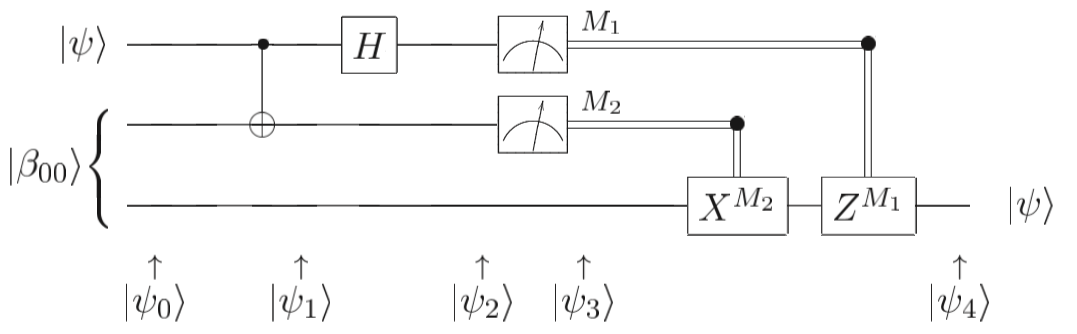
\includegraphics[width=0.6\textwidth]{continut/capitol1/figuri/TeleportationCircuit.png}
    \caption{Circuitul pentru teleportarea unui qubit. Nu voi explica ce înseamnă acest lucru, contează doar cum arată un circuit oarecare.}
    \label{fig:CircuitOarecare}
\end{figure}

Așadar, evoluția sistemului cuantic se interpretează de la stanga spre dreapta; în stânga față de fiecare linie care reprezintă starea fiecărui qubit individual se notează starea inițială a acelui qubit. Deseori, această stare este $\ket{0}$. Porțile logice cuantice pentru qubiți individuali sunt marcați sub forma unui dreptunghi cu un simbol reprezentativ în interior, iar cele care actionează asupra mai multor qubiți sunt reprezentați în diferite feluri, dar fac întotdeauna legătura între liniile mai multor qubiți. Liniile simple sunt pentru qubiți iar liniile duble sunt pentru biți clasici. Simbolul cu un "metru" reprezintă operația de măsurare.

Cea mai și cea mai importantă poartă logică cuantică pentru această lucrare este poarta Hadamard. Poarta Hadamard, față de porțile Pauli (prezentate în anexe), ne permit să ne îndepartăm de polii sferei Bloch și să obținem o superpoziție de $\ket{0}$ și $\ket{1}$. Transformarea Hadamard este definită prin:
\[
H\ket{0} = \frac{1}{\sqrt{2}} \ket{0} + \frac{1}{\sqrt{2}}\ket{1} = \ket{+},
\]
\[
H\ket{1} = \frac{1}{\sqrt{2}} \ket{0} - \frac{1}{\sqrt{2}}\ket{1} = \ket{-}.
\]

Iar reprezentarea matriceală a transformării Hadamard este 
\[
H = \frac{1}{\sqrt{2}}\begin{bmatrix}
1 & 1 \\
1 & -1
\end{bmatrix}
\]

De asemenea, transfomarea Hadamard poate fi exprimată ca o rotație de 90 grade în jurul axei Y, urmată de o rotație de 180 grade în jurul axei X, notat
\[
H = XY^{1/2},
\]
unde X și Y sunt porțile Pauli, notația cu exponent $\frac{1}{2}$ reprezentând o jumătate de rotație.

Efectul porții Hadamard:
\begin{figure}[!htb]
\minipage{0.5\textwidth}
  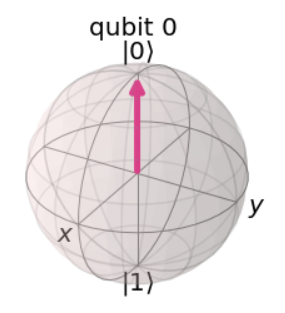
\includegraphics[width=\linewidth]{continut/capitol1/figuri/BlochDefault.png}
  \caption{Starea unui qubit inițializat în $\ket{0}$}\label{fig:bloch_default1}
\endminipage\hfill
\minipage{0.5\textwidth}
  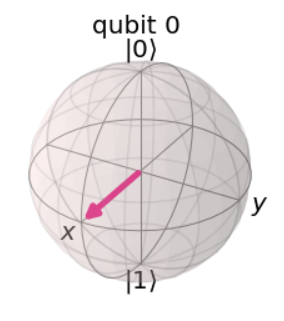
\includegraphics[width=\linewidth]{continut/capitol1/figuri/BlochHadamard.png}
  \caption{După aplicarea transformării Hadamard}\label{fig:bloch_hadamard}
\endminipage\hfill
\end{figure}

Așadar, cum amplitudinile cuantice $\alpha$ și $\beta$ din definiția qubitului sunt, după aplicarea porții Hadamard, amândouă $\frac{1}{\sqrt{2}}$, probabilitatea de obține fiecare dintre cele două stări, $\ket{0}, \ket{1}$ după măsurare este $(\frac{1}{\sqrt{2}})^2$, adică exact 1/2! Acest lucru practic trivializează conceptul fundamental a lucrării de față, adică acela de a realiza un generator de numere aleatorii folosind calculul cuantic, deoarece o simplă aplicare a porții Hadamard obține generarea unui număr cuantic exact uniform! Totuși, în capitolele următoare, voi realiza mai multe metode de generare a numerelor aleatorii cuantice și voi încerca să le demonstrez corectitudinea (adică, numerele generate sunt cu adevărat aleatorii) și să le măsura performanțele. În acest scop, pe lângă poarta Hadamard voi mai folosi următoarele porți:

\begin{itemize}
    \item Poarta de rotație generică în jurul axei y Ry
\end{itemize}
Ry este o poartă de rotație parametrizată. Reprezintă o rotație de $\theta$ radiani în jurul axei y. Trasformatea Ry este următoarea:
\[
R_y(\theta) = \begin{bmatrix}
\cos \frac{\theta}{2} & -\sin \frac{\theta}{2} \\
\sin \frac{\theta}{2} & \cos \frac{\theta}{2}
\end{bmatrix}
\]

În acest sens, pentru $\theta = \frac{\pi}{2}$, efectul acestei porți este exact același cu cel a unei porți Hadamard pentru un qubit inițializat în starea $\ket{0}$, fără "overhead"-ul unei rotații suplimentare în jurul axei x, lucru care, cum voi observa în capitolele următoare, are un efect relevant asupra performanței unui calculator cuantic!

\begin{itemize}
    \item Poarta de rotație generică U3
\end{itemize}

Aceasta este o poartă logică parametrizată care reprezintă o rotație cu 3 unghiuri Euler. Nu am găsit multă documentație despre aceasta, dar aceasta este deseori descompusă de fapt în câteva alte rotații:

\[
U3(\theta, \phi, \lambda) = RZ(\phi)RX(\phi/2)RZ(\theta)RX(\pi/2)RZ(\lambda),
\]
Unde $RX, RZ$ reprezintă porți generice de rotație în jurul axelor X, respectiv Z, similar cu poarta Ry descrisă anterior. De observat fapul că poarta U3 nu se folosește de o poartă Ry în descompunerea ei, motiv pentru care am analizat și performanța ei pentru generarea numerelor aleatorii. Reprezentarea matriceală a porții este următoarea:
\[
U3(\theta, \phi, \lambda) = \begin{bmatrix}
\cos\frac{\theta}{2} && -e^{i\lambda} \sin \frac{\theta}{2} \\
e^{i\phi}\sin \frac{\theta}{2} && e^{i(\phi + \lambda)} \cos \frac{\theta}{2}
\end{bmatrix}
\]

\section{Teste statistice}

Cum o mare parte din această lucrare se axează pe măsurarea performanțelor și corectitudinii mai multor metode de generare de numere aleatorii, mă voi utiliza de mai multe teste statistice pentru a verifica distribuțiile numerelor rezultate (voi testa uniformitatea numerelor generate în cazul scopului generării unei distribuții uniforme și normalitatea în cazul generării unei distribuții normale). Dar, înainte de a prezenta testele statistice, voi discuta câteva elemente de bază de statistică.

\subsection{Testarea ipotezelor statistice}

Formularea corectă de ipoteze statistice este probabil cel mai important aspect al cercetării din punct de vedere statistic. În acest sens, testarea statistică se face prin enunțarea a două ipoteze și apoi acceptarea (sau respingerea) ipotezei nulului:
\begin{itemize}
    \item Ipoteza nulului ($H_0$): reprezintă modelul pe care se dorește a se înlocui (respinge)
    \item Ipoteza alternativă ($H_1$): noul model, care în majoritatea cazurilor reprezintă negația ipotezei nulului.
\end{itemize}

Prin respingerea ipotezei nulului, se afirmă faptul că rezultatele nu sunt datorate întamplării și se poate spune că rezultatul obținut este seminificativ din punct de vedere statistic.

\subsection{Pașii unui test statistic}
\begin{itemize}
    \item Formularea problemei în termenii ipotezelor statistice,
    \item Alegerea unui test statistic și o metrică asociată potrivită pentru problemă
    \item Alegerea unui nivel de semnificație și apoi calcularea pragului de separare (valoarea critică) dintre valorile acceptabile și cele considerate inacceptabile (de obicei, o probabilitate de 95 sau 99\%),
    \item Calcularea parametrilor statistici folosind datele eșantionului
    \item Compararea valorii calculate cu valoarea critică pentru a decide dacă ipoteza nulului se respinge sau se acceptă.
\end{itemize}

\subsection{Valoarea p}

În statistică, valoarea p este probabilitatea obținerii de rezultate cel puțin la fel de extreme ca rezultatele observate ale unui test statistic, asumând că ipoteza nulului este corectă. Valoarea p, care inseamnă valoare a probabilității, este un instrument statistic de masură, cu valori cuprinse între 0 și 1. Este folosită în cadrul testării ipotetice. 

Valoarea p se calculeaza pornind de la deviația dintre o valoare observată și o valoare aleasă de referință, știind funcția densitate de probabilitate a statisticii, cu o diferență mai mare însemnând o valoare mai mică pentru valoarea p. 

Deci, valoarea p reprezintă probabilitatea ca efectele observate să fie la fel de mari ca cele din studiu. Dacă valoarea p este mică, rezultatele studiului nu se datorează intâmplării și respingem ideea că nu există nicio diferență între cele doua eșantionane (respingem ipoteza nulului). Dacă valoarea p este mare, diferențele observate se datorează cel mai probabil intâmplării și nu vom respinge ideea că nu există diferențe între eșantioane.

Valoarea p va fi utilizată deseori în această lucrare pentru a verifica corectitudinea respingerii ipotezelor enunțate de către mine.

\subsection{Testul Z pentru compararea mediilor a două eșantioane cu varianțe inegale}

Parametrul testului este
\[
z = \frac{\bar{X}_1 - \bar{X}_2}{\sqrt{\frac{s_1^2}{n_1} + \frac{s_2^2}{n_2}}},
\]
unde
\begin{itemize}
    \item $\bar{X_1}$ = media primului eșantion,
    \item $n_1$ = volumul primului eșantion,
    \item $s_1^2$ = varianța primului eșantion.
\end{itemize}
Idem pentru al doilea eșantion.
Comparând acest z calculat cu valoarea z dintr-un tabel al valorii z normale, se determină în acest fel regiunea critică a testului (bilateral sau unilateral) și se acceptă sau respinge ipoteza nulului în funcție semnul de comparare dintre valoarea calculată și cea din tabel.

\subsection{Testul Kologomorov-Smirnov}

Este un test neparametric pentru testarea egalității a două funcții de distribuție care poate fi utilizat pentru a compara un eșantion cu funcție de distribuție de referință sau a compara două eșantioane a căror distribuție nu se cunoaște. În acest sens, mă voi folosi de acest test pentru a compara rezultatul unei generări de numere aleatorii care să urmeze o distribuție normală (de exemplu, functia $randn()$ din Matlab) cu o distribuție normală cu aceeași parametri ca cei utilizați de distribuția dorită.

Din păcate, documentația pentru acest test este cam slabă, și nu prea am reușit să găsesc o metodă implementă în vreun limbaj de programare, așa că acest test este singurul pentru care mă voi folosi de o implementare nefăcută de mine. Singurul motiv pentru care fac acest lucru este deoarece sunt absolut sigur că acest test este cel mai potrivit pentru cerințele mele.

Parametrul testului pentru o funcție cumulativă de distribuție $F(x)$ este
\[
D_n = \sup_x |F_n(x) - F(x)|,
\]
unde $\sup_x$ este supremum-ul setului de distanțe. Intuitiv, statistica ia cea mai mare diferență în modul a celor două funcții de distribuție pentru toate valorile $x$.

\subsection{Alte măsurători relevante pentru uniformitatea numerelor aleatorii}
În următoarele câteva subsecțiuni voi prezenta cele câteva măsurători pentru uniformitatea numerelor aleatorii propuse în \cite{art:PetrilaMantaUnguranu:IEEESystheory:2014}.
\subsubsection{Media distribuției}

Un simplu test cantitativ pentru uniformitate este dată de media numerelor aleatorii,
\[
\bar{u_n} = \frac{1}{N}\sum^N_{n=1}u_n.
\]
Care ar trebui întotdeauna să fie aproximativ egală cu
\[
\int_0^1xdx = \frac{1}{2}.
\]

\subsubsection{Parametrul Pearson chi-pătrat}

Pentru a testa uniformitatea, statistica chi-pătrat este definită ca
\[
\chi^2 = \frac{K}{N(K-1)}\sum^K_{i=1}(n_i - N/K)^2,
\]
unde K este numărul de subintervale în care distribuția a fost partiționată și cu $n_i$ numărul de valori în subintevalul $i$.

\subsubsection{Coeficientul de corelație și forma simplificată}

Un alt test important pentru măsurarea calității generatorului de numere aleatorii este testul de corelație între numere succesive generate de acesta. Luând în considerare fiecare pereche de două numere succesive generate de generator, se definește coeficientul de corelație:
\[
C = \frac{N\sum^N_{n=2}(u_n-\bar{u})(u_{n-1}-\bar{u})}{(N-1)\sum^N_{n=1}(u_n-\bar{u})^2}
\]
Coeficientul de corelație $C$ redă informații relevante despre conexiunile dintre diferite subseturi de date. Acest coeficient ar trebui să tindă la valoarea 0.

Totuși, după cum se poate observa, în această definiție, numitorul este un  termen de uniformizare. Astfel, expresia poate să nu descrie exclusiv corelația, fiindcă depinde de uniformitatea numerelor aleatorii. Cum numitorul, în general, este un termen de normalizare, corelația poate fi descrisă pur și simplu de media aritmetică a perechilor de numere succesive,
\[
u_n u_{n-1} = \frac{1}{N-1}\sum^N_{n=2}u_n u_{n-1},
\]
care ar trebui întotdeauna să tindă la
\[
\int_0^1 \int_0^1 xydxdy = \frac{1}{4}
\]
pentru numere necorelate. 
\pagebreak
\section{Numerele aleatorii, generatorarele de numere pseudoaleatorii și proprietățile lor}
\subsection{Definiția numerelor aleatorii și teste de aleatoritate}
Un număr aleator este un număr generat printr-o metodă oarecare care face parte dintr-un set care prezintă \textit{aleatoritate statistică}. O secvență de numere poate fi numită drept \textit{aleatorii} din punct de vedere statistic dacă nu urmează un anumit tipar sau șablon și nu prezintă regularități sau periodicitate. De exemplu, variabila rezultată prin aruncarea unui zar netrucat și memorizarea rezultatelor se poate numi drept aleatorii statistic. 

M.G. Kendall și B. Babington Smith prezintă în \cite{MGKendallBBSmithRandomness}
conceptele de numere \textit{local} aleatorii, în contrast cu conceptul de numere \textit{global} aleatorii. Un set de numere este "global" aleator dacă pentru o cantitate suficientă de numere secvența pare a fi aleatorii, chiar dacă anumite subsecvențe nu par a fi deloc aleatorii. De exemplu, într-un set suficient de mare de numere aleatorii, pot apărea secvențe lungi de același număr, acest lucru nedescalificând setul de la proprietatea de "aleatoritate". Un set de numere este "local" aleator dacă există o secvență de lungime minimă prin care distribuția este aproximată. Practic, un set de numere este local aleator dacă nu prezintă proprietățile descrise pentru numerele global aleatorii. 

Aceste lucruri sunt relevante deoarece există, de exemplu, regulații în industria jocurilor de noroc care interzic existența de subsecvențe lungi de același număr generat de o mașinărie, lucru care implică necesitatea existenței aleatorității locale.

Kendall și Smith prezintă patru teste bazate pe ipoteză cu ipoteza nulului fiind că toate numerele într-o secvență aleatorie au o probabilitate egală de a apărea, și că mai multe alte șabloane din setul de date ar trebui să fie, de asemenea, echiprobabile.

Aceste teste propuse sunt:
\begin{itemize}
    \item Testul de frecvență - Un test foarte simplu, pe care îl voi folosi excesiv pe parcursul lucrării, și anume verificarea că numerele dintr-o secvență de date apar cu probabilitate aproximativ urmând o distribuție dată (în cazul meu, o distribuție uniformă sau una normală);
    \item Testul serial - Un test similar cu cel de frecvență, dar care folosește perechi de câte două numere pentru a verifica urmărirea unei distribuții de către secvența de date;
    \item Testul "poker" - Testează secvențe de câte cinci numere odată, similar cu testarea pentru o mână de poker;
    \item Testul "gap" sau de interval - Testează, în lucrarea autorilor, intervalul dintre oricare două zero-uri, dar se poate generaliza pentru intervalul dintre oricare două numere din universul numerelor posibile de generat.
\end{itemize}

Pe lângă testele statistice bazate pe ipoteză descrise anterior, mă voi folosi și de aceste teste frecventiste, în special datorită ușurinței de prezentare a unor vizualizări utile pentru acestea (adică, voi arăta și distribuția numerelor generate, pentru testul de frecvență, de exemplu).

\subsection{Alte proprietăți ale generatoarelor de numere pseudoaleatorii}

Patru proprietăți esențiale ale numerelor aleatorii sunt:
\begin{itemize}
    \item Repetabilitate: în aceleași condiții de generare, un generator ar trebui să producă același set de numere. Altfel spus, generatoarele de numere pseudoaleatorii trebuie să producă același set de numere pentru un seed inițial anume;
    \item Aleatoritate: generatorul trebuie să treacă cel puțin testele descrise anterior, dar sunt mult mai multe teste de aleatoritate;
    \item O perioadă lungă: secvențele de numere pseudoaleatorii se folosesc de aritmetică cu precizie finită, deci secvența trebuie să se repete cu o perioadă finită. Această perioadă trebuie să fie cu mult mai mare față de numărul de numere necesar pentru un experiment dat;
    \item Lipsa de sensibilitate față de seed: proprietățile de aleatoritate ale generatorului nu ar trebui să depindă de seed-ul acestuia.
\end{itemize}

\subsection{Entropia}

Entropia este o unitate de măsură a incertitudinii unui sistem. O entropie bună provine din mediul înconjurător al sistemului și este reprezentat de lipsa predictibilității și, în general, de haos. Un HRNG (Hardware Random Number Generator) se folosește de valori greu de ghicit, precum măsurători de presiune atmosferică sau valori de viteză a vântului, dar în cazul sistemelor de calcul se folosesc deseori fenomene haotice și imprevizibile, precum mișcarea cursorului, tastele apăsate de un utilizator, dar și viteze de scriere a disk-ului sau viteze de transfer prin rețea. 

Începând cu anul 2012, procesoarele intel care folosesc arhitectura Ivy Bridge sau mai nou conțin un HRNG bazat pe guideline-urile NIST SP 800-90 \footnote{https://csrc.nist.gov/publications/detail/sp/800-90a/rev-1/final}. Intel oferă instrucțiuni la nivelul limbajului de asamblare, dar pe sistemele de operare Linux se poate interacționa cu circuitul HRNG prin intermediul dispozitivului /dev/hwrng. 


\subsection{Metode clasice de generare a numerelor aleatorii}

\subsubsection{Metoda LCG}

Metoda LCG (Linear Congruential Generator) este un algoritm care produce o secvență de numere pseudoaleatorii calculată cu o ecuație liniară pe porțiuni. Metoda este unul dintre cei mai vechi și utilizați algoritmi de generare de numere pseudoaleatorii. Motivația popularității metodei este utilizarea de instrucțiuni ușor de implementat și utilizat de către sistemele de calcul. 

Generatorul este definit de funcția de recurență 
\[
X_{n+1} = (aX_n + c) \enspace mod \enspace m
\]
unde $X$ este secvența de numere pseudoaleatorii, $m$ este "coeficientul" sau "modulus"-ul, $a$ este înmuțitorul, $c$ este "increment"-ul iar $X_0$ este "seed"-ul sau valoarea de start a generatorului. Pentru o valoare $c = 0$, generatorul poate fi numit de fapt Multiplicative Congruential Generator (MCG). Teoretic, pentru un $c \neq 0$, funcția de recurență ar trebui defapt denumită "transformare afină" și nu "liniară", dar se păstrează denumirea de "liniară" din motive istorice.

Un beneficiu principal a metodei LCG este faptul că, pentru niște parametri aleși corespunzător, se pot obține valori de periodicitate foarte mari și periodicitatea rămâne cunoscută. 

Specific, în aplicația mea, voi folosi un LCG care îndeplinește cerințele teoremei Hull-Dobell, enunțată în \cite{HullDobellRNGs}, cerințele acestei teoreme fiind:
\begin{itemize}
    \item $m$ și $c$ sunt numere coprime;
    \item $a-1$ este divizibilă cu toți factorii primi ai lui $m$;
    \item $a-1$ este divizibilă cu 4 dacă $m$ este divizibil cu 4.
\end{itemize}

Îndeplinirea cerințelor teoremei Hull-Dobell asigură faptul că generatorul va avea perioada maximă posibilă, egală cu $m$, indiferent de valoarea de start (seed-ul). 


Pentru următoarele câteva generatoare pe care le voi prezenta nu există multă documentație datorită publicării acestora original pe newsgroup-uri de usenet, între anii 1996 și 2011, de către autorul George Marsaglia \cite{misc:usenet:GeorgeMarsaglia}. Pentru generatoarele CONG, SHR3 și MWC, voi prezenta doar formulele lor de calcul. 

\subsubsection{Generatorul CONG}

Pentru generatorul CONG (Congruential Generator), se folosește relația de recurență
\[
X_{n+1} = 69069 \cdot X_{n} + 1234567.
\]
Valorile pentru înmulțitor și increment, anume 69069 și 1234567 au fost alese de către George Marsaglia. Aparent înmulțitorul de 69069 era foarte popular în 1996. Generatorul are o perioadă de $2^{32}$. Autorul spune că deși primii 16 biți trec cu brio testele de aleatoritate, ultimii 16 sunt "prea regulați". Autorul sugerează utilizarea generatorului CONG (care deja era utilizat pe sistemele Delphi) împreună cu un alt generator.

\subsubsection{Generatorul MWC}

Pentru generatorul MWC (Multiply With Carry) se concatenează două numere pe 16 biți cu relațiile de recurență
\[
X_n = 36969 \cdot X_{n-1} + carry, 
\]
\[
Y_n = 18000 \cdot Y_{n-1} + carry
\],
totul modulo $2^{32}$. Are o perioadă de $2^{60}$ și aparent era un preferat în industrie la momentul scrierii.

\subsubsection{Generatorul SHR3}

Pentru generatorul SHR3 (3 Shift Register Generator), se folosește relația 
\[
Y_n = Y_{n-1} (I + L \XOR 17) (I + R \XOR 13) (I + L \XOR 5) 
\]
, unde "$\XOR$" reprezintă operația XOR pe biți. Pentru valorile pentru I, L și R voi folosi valorile din implementarea oferită de autor.

\subsubsection{Generatorul KISS}

Generatorul KISS (Keep It Simple, Stupid, sau, cenzurat, "Sir") se folosește de toate celelalte generatoare de numere pseudoaletorii prezentate până acum (CONG, MWC și SHR3) în felul următor:
\begin{figure}[H]
    \centering
    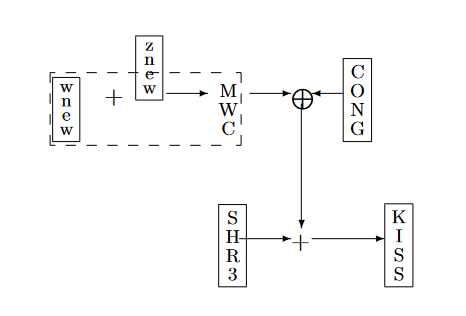
\includegraphics{continut/capitol1/figuri/KissDiagram.png}
    \caption{Diagrama logică a generatorului KISS}
    \label{fig:GeneratorKissDiagrama}
\end{figure}

Blocurile "znew" și "wnew" reprezintă de fapt numerele I, L și R prezentate anterior. Are o perioadă de $2^{123}$ și este una dintre preferatele autorului, deși între timp s-au descoperit mai multe probleme cu acest generator \cite{KISSABitTooSimple}. Totuși, pe acesta îl voi implementa și eu, pentru a realiza mai multe teste pe numere pseudoaleatorii. Figură preluată din \cite{KISSABitTooSimple}.

\section{Specificațiile aplicației}

Tot ce am prezentat până în acest moment sunt elemente teoretice necesare explicării corecte a specificațiilor aplicației mele. Prin urmare, scopul urmărit de mine este atât design-ul unor circuite cuantice care să poată fi implementate pe un calculator cuantic adevărat (codul va fi executat, într-o anumită etapă, și folosind un serviciu Cloud de quantum computing pentru a executa experimentele cuantice pe un calculator cuantic adevărat), cât și studiul corectitudinii generării numerelor, prin metode statistice descrise anterior, dar și măsurarea performanțelor multiplelor metode și circuite analizate, în diferite cazuri de utilizare. 
Așadar, pe scurt, aplicațiile lucrării vor face următoarele:
\begin{itemize}
    \item Vor prezenta circuitele cuantice utilizate pentru generarea de o distribuție aleatorii uniformă și una normală;
    \item Vor analiza corectitudinea generării acestor numere, prin metode statistice;
    \item Vor analiza performanțele metodelor de generare;
    \item Va exista și o aplicație cu interfață utilizator pentru expunerea funcționalițății analizate (dar nu neapărat și cele de analiză statistică etc.).
\end{itemize}




